\documentclass[a4paper]{article}

\usepackage[utf8]{inputenc}

%  General style files
\usepackage{fancybox}%         e.g. for calling out requirements, etc.
\usepackage{multicol}%         multiple columns (e.g. glossary)
\usepackage{longtable}% GOA: added 1 Jun 2007 for Christos
\usepackage{array}%
\usepackage{lineno}%           Does line numbers in margins (see \linenumbers command)

% Override the (rather clunky) default fonts of LaTex throughout
\usepackage{palatino}      % Choose default roman font.  Others are times, pslatex, newcent, bookman, chancery
\usepackage{mathpazo}      % Matching math fonts (see http://www.math.uiuc.edu/~hartke/computer/latex/survey/survey.html)
\usepackage{helvet}        % Choose default sans serif
\usepackage{sectsty}       % Change style of headings (should precede section redefinitions below)
\allsectionsfont{\sffamily}% Set sans serif for all headings

\usepackage{fancyhdr}%        modern version of fancyheadings
\usepackage{subfig}%
\let\subfigure\subfloat% compatibility between subfigure and subfig packages
\usepackage{xspace}%
\usepackage{multirow}%
\usepackage{dcolumn} % for aligning columns on decimal: rather picky

\usepackage[table,usenames,dvipsnames]{xcolor}% just for warnings so far; do not use for journal submission without prior approval


\usepackage[bookmarksnumbered,bookmarksopen,bookmarksopenlevel=1,colorlinks=false,pdfborder={0 0 0},plainpages=false,pdfpagelabels]{hyperref}


%%%%%%%%%%%%%%%%%%%%%%%%%%%%%%%%%%%%%%%%%%%%%%%%%%%%%%%%%%%%%%%%%%%%
% Define the default parskip so it can be reset back to this after
% it is locally changed in other environments
\newlength{\parskipsaved}
\setlength{\parskipsaved}{0.5\baselineskip}

% Define page layout
\setlength{\textwidth}{160mm}
\setlength{\textheight}{235mm}
\setlength{\columnsep}{10mm}
\setlength{\columnseprule}{0.3pt}% if zero then there is no rule between 2 columns

\if@twoside
  \setlength{\oddsidemargin}{0mm}
  \setlength{\evensidemargin}{0mm}
\else
  \setlength{\oddsidemargin}{0mm}
  \setlength{\evensidemargin}{0mm}
\fi

\setlength{\footskip}{36pt}
\setlength{\headheight}{25pt}
\setlength{\headsep}{20pt}%     Distance from bottom of header to main body
\setlength{\topmargin}{-8pt}

% Margin notes
\setlength{\marginparpush}{\baselineskip}% space between successive notes
\setlength{\marginparsep}{3mm}%            distance from main text
\setlength{\marginparwidth}{20mm}%         width of note

% Paragraph spacing / indentation
\setlength{\parindent}{0pt}
\setlength{\parskip}{\parskipsaved}

\raggedbottom

%%%%%%%%%%%%%%%%%%%%%%%%%%%%%%%%%%%%%5
% My Stuff
%%%%%%%%%%%%%%%%%%%%%%%%%%%%%%%%%%%%%5
\usepackage{colortbl}
\usepackage{graphicx}
\usepackage{ulem}
\usepackage{listings}
\usepackage[toc,page]{appendix}
\usepackage{epstopdf}
\usepackage{framed}  % Boxes around stuff
\usepackage{siunitx} % Allows easy x10^ for numbers

% title, author and date
\title{QCD Samples with VBF-like jets and MET - Feasibility Study for Run II} 
\author{Joao Pela\\
 Imperial College London\\
   \texttt{joao.pela@cern.ch}}
\date{\today}

\begin{document}

\maketitle

\begin{abstract}
Study on the feasibility of QCD samples with VBF-like jets and MET characteristics to be used in the CMS VBF Higgs to Invisible analsysis during the LHC Run II period. This study will cover cost (physics usability, computing and disk storage) of several possibilities to make such samples.
\end{abstract}

\section{Introduction}

Simulating and reconstructing quantities of QCD events in quantities comparable to the ones produced at the LHC experiments is impractical. At every second of LHC physics operation 
several million bunch crossings happen each one containing several collisions. With current hardware it takes in excess of one minute to fully simulate one of such bunch crossings. This constraints lead to QCD events being simulated in $p_\perp$ hats, where the first collision is generated in a specific $p_\perp$ range and then several other collision are added as pile-up. This extra collisions are generated without any constraints in $p_\perp$. 

This bin method allows the user to have samples with increasing energy and study the influence of each of them in their own analysis. As a practical example a user does not need to look over millions of events to find high energy jets, he can just test the higher $p_\perp$ hats as needed.

On the other hand, there are some analysis that require jets and/or MET with very low values where this inclusive QCD samples will not have enough statistics to provide insight into the QCD behaviour. The CMS VBF Higgs to invisible is one of such analysis.

During the preparation the Run I VBF Higgs to invisible analysis a set of QCD samples with VBF like jets and real MET was generated. This samples allowed to understand the mechanisms that create real MET in QCD and how those could be mitigated.

The analysis is now preparing for Run II it was considered once again to be useful to have similar samples remade and possibly extended. It was identified that not only real MET is significant but also fake MET coming from detector miss measurement and as such a sample that could simulate such effects would be of great interest.

This study investigates the alternatives and attempts to quantify the costs of of producing such samples.

\section{Objectives and methods}

The objective of this study is to identify possible working points for the production of QCD samples with VBF-like jets and MET. 

Since this type of events is very rare, we need to filter this events in order to have manageable sample sizes. There are also computing limitations, while running a Monte Carlo generator is not very costly in terms of CPU time, running the full CMS simulation is.

Steps where filters can be inserted:
\begin{itemize}
 \item Monte Carlo Generation
 \item Level 1 Trigger
 \item High Level Trigger
 \item Offline
\end{itemize}

To maximise physics usability of this samples the one should consider:
\begin{itemize}
  \item Avoid any cut on generator level MET, in order to pick up fake MET events.
  \item Samples should be of similar size to the inclusive QCD samples
  \item $\Delta\phi(jet-jet)$ cuts should be avoided since the Run I analysis uses inverted cuts in this variable on a data-driven QCD estimation.
\end{itemize}

\section{Cross section}

The cross section for each QCD $p_\perp$ hat at 

\begin{table}[htp]
\centering

\begin{tabular}{|c|c|c|c|}
\hline
 & \multicolumn{3}{c|}{Cross Section [pb]} \\
\hline
$p_\perp$ hat [GeV] & 8 TeV & 13 TeV & Change \\
\hline
\hline
30-50   & 66285328      & 161500000.   & +243.6\% \\
50-80   &  8148778.0    &  22110000.   & +271.3\% \\
80-120  &  1033680.0    &   3000114.3  & +290.2\% \\
120-170 &   156293.3    &    493200.   & +315.6\% \\
170-300 &    34138.15   &    120300.   & +352.4\% \\
300-470 &     1759.549  &      7475.   & +424.8\% \\
470-600 &      113.8791 &       587.1  & +515.5\% \\
600-800 &       26.99   &       167.   & +618.7\% \\
\hline
\end{tabular}

\end{table}



As expected the cross section increase significantly from 8 TeV to 13 TeV and this effect becomes more and more significant as you go up in $p_\perp$ hat.

\begin{table}
\centering

\begin{tabular}{|c|c|c|c|}
\hline
pT Hat &  X-Section (pb) &  10 fb-1 & 30 fb-1 \\
\hline
\hline
  30-50 & \num{1.62E+08} & \num{1.62E+12} & \num{4.85E+12} \\
  50-80 & \num{2.21E+07} & \num{2.21E+11} & \num{6.63E+11} \\
 80-120 & \num{3.00E+06} & \num{3.00E+10} & \num{9.00E+10} \\
120-170 & \num{4.93E+05} & \num{4.93E+09} & \num{1.48E+10} \\
170-300 & \num{1.20E+05} & \num{1.20E+09} & \num{3.61E+09} \\
300-470 & \num{7.48E+03} & \num{7.48E+07} & \num{2.24E+08} \\
470-600 &          587.1 & \num{5.87E+06} & \num{1.76E+07} \\
600-800 &            167 & \num{1.67E+06} & \num{5.01E+06} \\
\hline
\end{tabular}


\caption{Quantity of event for each of the studied QCD $p_\perp$ hats for 10 and 30 $fb^-1$ of integrated luminosity.}
\label{table_QCD_RunII_EventsIntegratedLuminsity}
\end{table} 


\section{Run I VBF QCD samples characteristics}

In the section we will summarize the characteristics of VBF QCD samples produced for the Run I analysis.

Two filters were applied to data, one over the generator level met and another over generator level jets. Here, generator level MET is defined as the vectorial sum of the $p_\perp$ of all neutrinos on the event. The implemented filters selected events according to the following characteristics:

MC Filter: Vectorial sum of neutrino $E_T$
\begin{itemize}
  \item $\sum E_\perp(\vec{\nu}) > 40$ $GeV$
\end{itemize}

MC Filter: Dijet Filter
\begin{itemize}
  \item Select jets with:
  \begin{itemize}
    \item $p_\perp>20$ $GeV$
    \item $|\eta|<5.0$
  \end{itemize}
  \item From selected jets at least one pair with:
  \begin{itemize}
    \item $m_{jj}>700$ $GeV$
    \item $\Delta\eta>3.2$
  \end{itemize}    
\end{itemize}

By applying this filters we were able to pass only a small fraction of the events to the detector simulation.

\begin{table}
\centering

\begin{tabular}{|c|r|c|r|c|c|}
\hline
$p_\perp$ Hat & Ev. Gen. & Filter Eff. &  Events &  XS $[pb]$ & Eq. Lumi. $[fb^{-1}]$ \\
\hline \hline
80-120  & 39376000000 &    0.000049 & 1614416 &  1033680 &  38.09 \\
120-170 &  7000000000 &    0.000283 & 2051000 & 156293.3 &  44.79 \\
170-300 &  1375000000 &    0.000987 & 1391500 & 34138.15 &  40.28 \\
300-470 &    80000000 &    0.002659 &  207840 & 1759.549 &  45.47 \\
470-600 &    25000000 &    0.004127 &  104675 & 113.8791 & 219.53 \\
\hline
\end{tabular}

\caption{TODO}
\label{table_RunI_QCDFiltered_FilterEff}
\end{table}

The resulting samples were publish in the CMS physics analysis database with url:

\begin{center}
https://cmsdbsprod.cern.ch:8443/cms\_dbs\_ph\_analysis\_01\_writer/servlet/DBSServlet
\end{center}

With the following database names:
 
\begin{table}
\centering
 
\resizebox{\linewidth}{!}{
\begin{tabular}{|c|l|}
\hline
$p_\perp$ hat & Identifier \\
\hline \hline
80-120  & /VBFQCD\_Pt\_80to120\_MET40\_step1\_v1/pela-VBFQCD\_Pt\_80to120\_MET40\_step3\_v1-3664d28163503ca8171ba37083c39fc9/USER \\
120-170 & /VBFQCD\_Pt\_120to170\_MET40\_step1\_v1/pela-VBFQCD\_Pt\_120to170\_MET40\_step3\_v1-3664d28163503ca8171ba37083c39fc9/USER \\
170-300 & /VBFQCD\_Pt\_170to300\_MET40\_step1\_v1/pela-VBFQCD\_Pt\_170to300\_MET40\_step3\_v1-3664d28163503ca8171ba37083c39fc9/USER \\
300-470 & /VBFQCD\_Pt\_300to470\_MET40\_step1\_v1/pela-VBFQCD\_Pt\_470to600\_MET40\_step3\_v1-3664d28163503ca8171ba37083c39fc9/USER \\
470-600 & /VBFQCD\_Pt\_470to600\_MET40\_step1\_v1/pela-VBFQCD\_Pt\_470to600\_MET40\_step3\_v2-3664d28163503ca8171ba37083c39fc9/USER \\
\hline
\end{tabular}
}

\caption{TODO}
\label{table_RunI_QCDFiltered_SampleNames}
\end{table}



\section{Phys14 QCD samples}

Before we start investigating possible production filters we need to define a baseline production. For this purpose, the Phys14 samples were chosen since this production was fairly recent and this samples were tested in a CMS wide exercise. Some details about this samples can be found in the table \ref{table_QCD_Phys14DR_SampleDetails}.

\begin{table}[htp]
\centering

\resizebox{1.0\linewidth}{!}{
\begin{tabular}{|l|c|}
\hline
Dataset & Sample Size \\
\hline
\hline
/QCD\_Pt-30to50\_Tune4C\_13TeV\_pythia8/Phys14DR-AVE30BX50\_tsg\_castor\_PHYS14\_ST\_V1-v2/AODSIM   & 5M \\
/QCD\_Pt-50to80\_Tune4C\_13TeV\_pythia8/Phys14DR-AVE30BX50\_tsg\_castor\_PHYS14\_ST\_V1-v1/AODSIM   & 5M \\
/QCD\_Pt-80to120\_Tune4C\_13TeV\_pythia8/Phys14DR-AVE30BX50\_tsg\_castor\_PHYS14\_ST\_V1-v1/AODSIM  & 5M \\
/QCD\_Pt-120to170\_Tune4C\_13TeV\_pythia8/Phys14DR-AVE30BX50\_tsg\_castor\_PHYS14\_ST\_V1-v1/AODSIM & 5M \\
/QCD\_Pt-170to300\_Tune4C\_13TeV\_pythia8/Phys14DR-AVE30BX50\_tsg\_castor\_PHYS14\_ST\_V1-v1/AODSIM & 3M \\
/QCD\_Pt-300to470\_Tune4C\_13TeV\_pythia8/Phys14DR-AVE30BX50\_tsg\_castor\_PHYS14\_ST\_V1-v1/AODSIM & 3M \\
/QCD\_Pt-470to600\_Tune4C\_13TeV\_pythia8/Phys14DR-AVE30BX50\_tsg\_castor\_PHYS14\_ST\_V1-v1/AODSIM & 3M \\
/QCD\_Pt-600to800\_Tune4C\_13TeV\_pythia8/Phys14DR-AVE30BX50\_tsg\_castor\_PHYS14\_ST\_V1-v1/AODSIM & 3M \\
\hline
\end{tabular}
}

\caption{Details on the inclusive QCD samples produces for the Phys14 exercise. Only the samples with average pile-up 30 and 50 ns separation are showed.}
\label{table_QCD_Phys14DR_SampleDetails}
\end{table}


This samples were produced with CMSSW\_7\_2\_0\_patch1. We will be using the same version for this study since any produced test samples can be tested with the same receipts used to analyse Phys14 samples.

Unfortunately, it was found that this QCD samples were not created from scratch. They are simply a reprocessing of previously produced samples produce in the Fall13 campaign with CMSSW\_6\_2\_0\_patch1. This means we cannot simply use the same configuration files used to produce Phys14 samples since this will not run any Monte Carlo generator but only re-process existing samples.  

\section{QCD pT hat characteristics}

% Plots need relooking
\begin{minipage}{.5\textwidth}
  \centering
  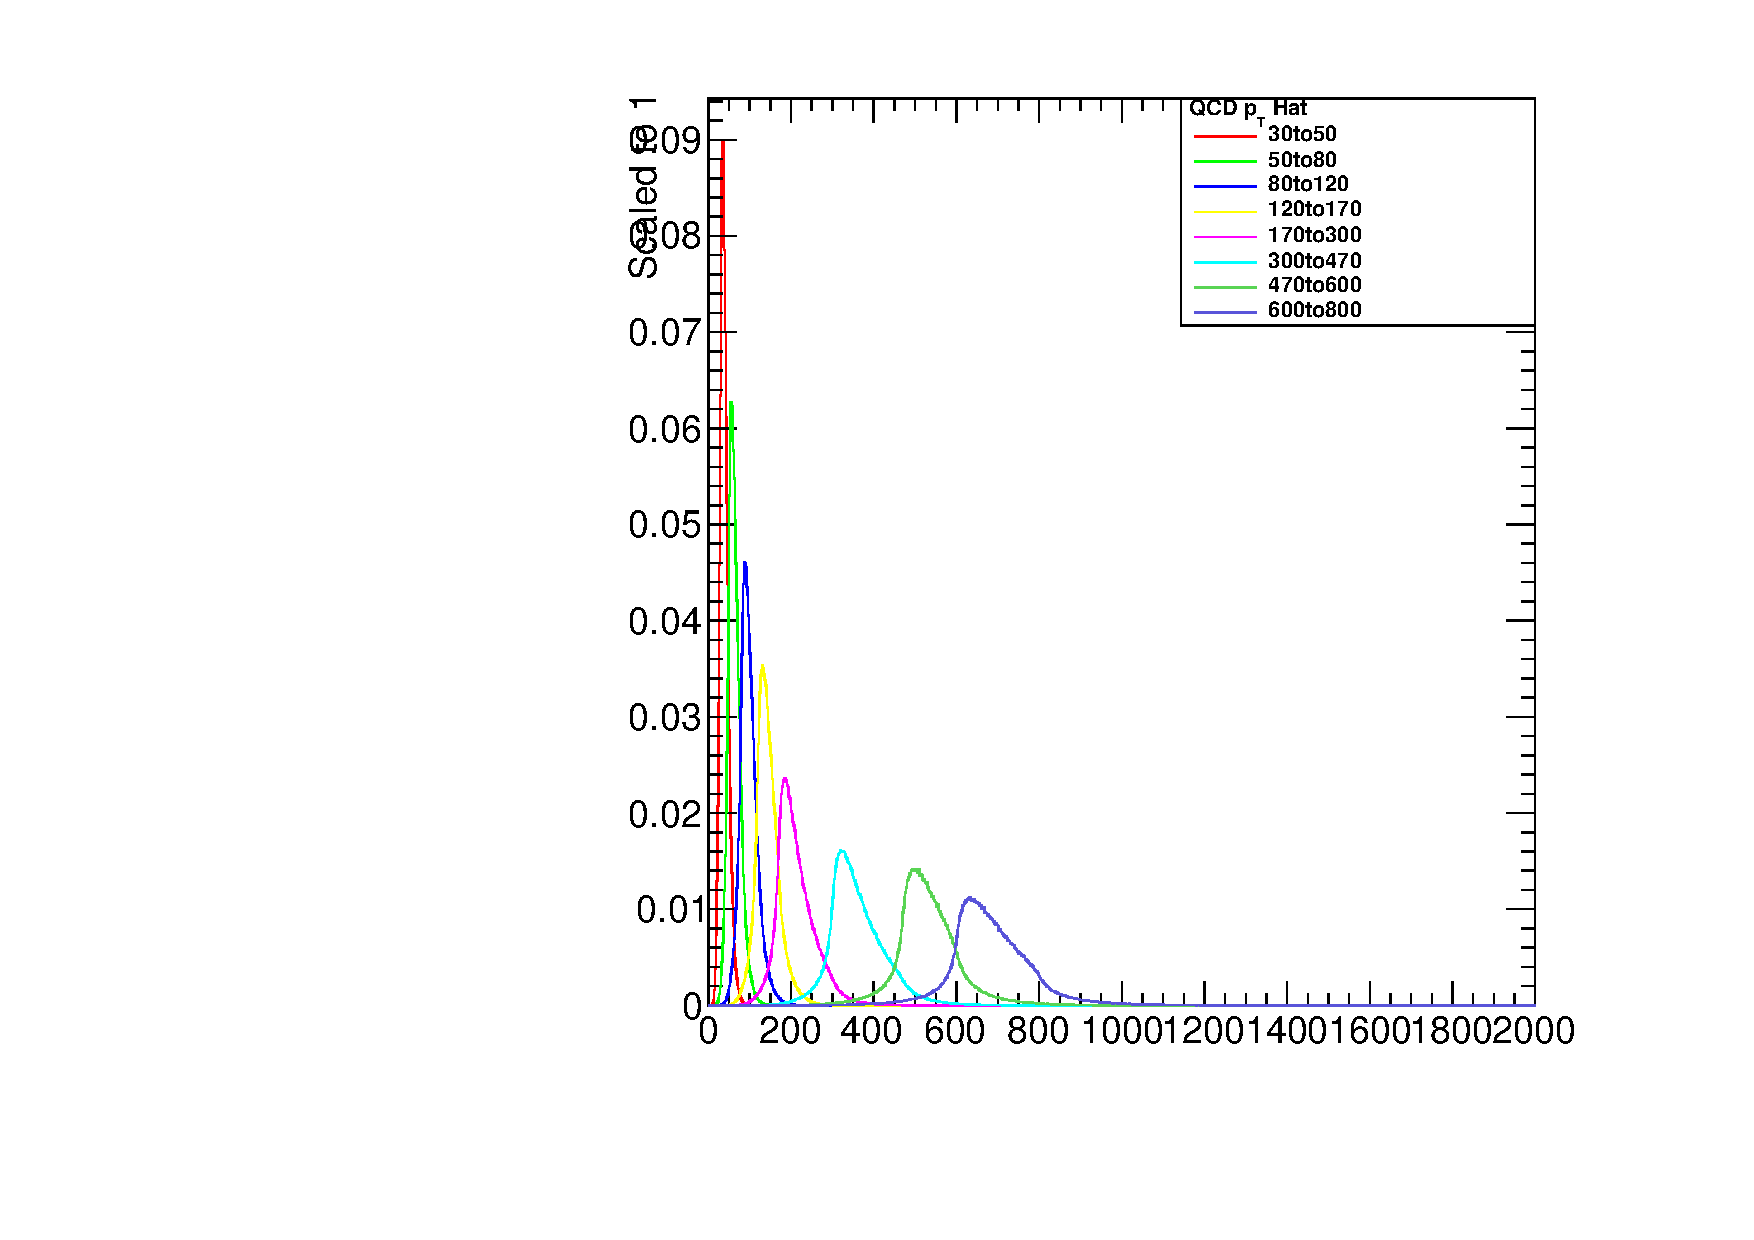
\includegraphics[width=1.0\linewidth]{img/Jet0_Pt.pdf}
\end{minipage}%
\begin{minipage}{0.5\textwidth}
  \centering
  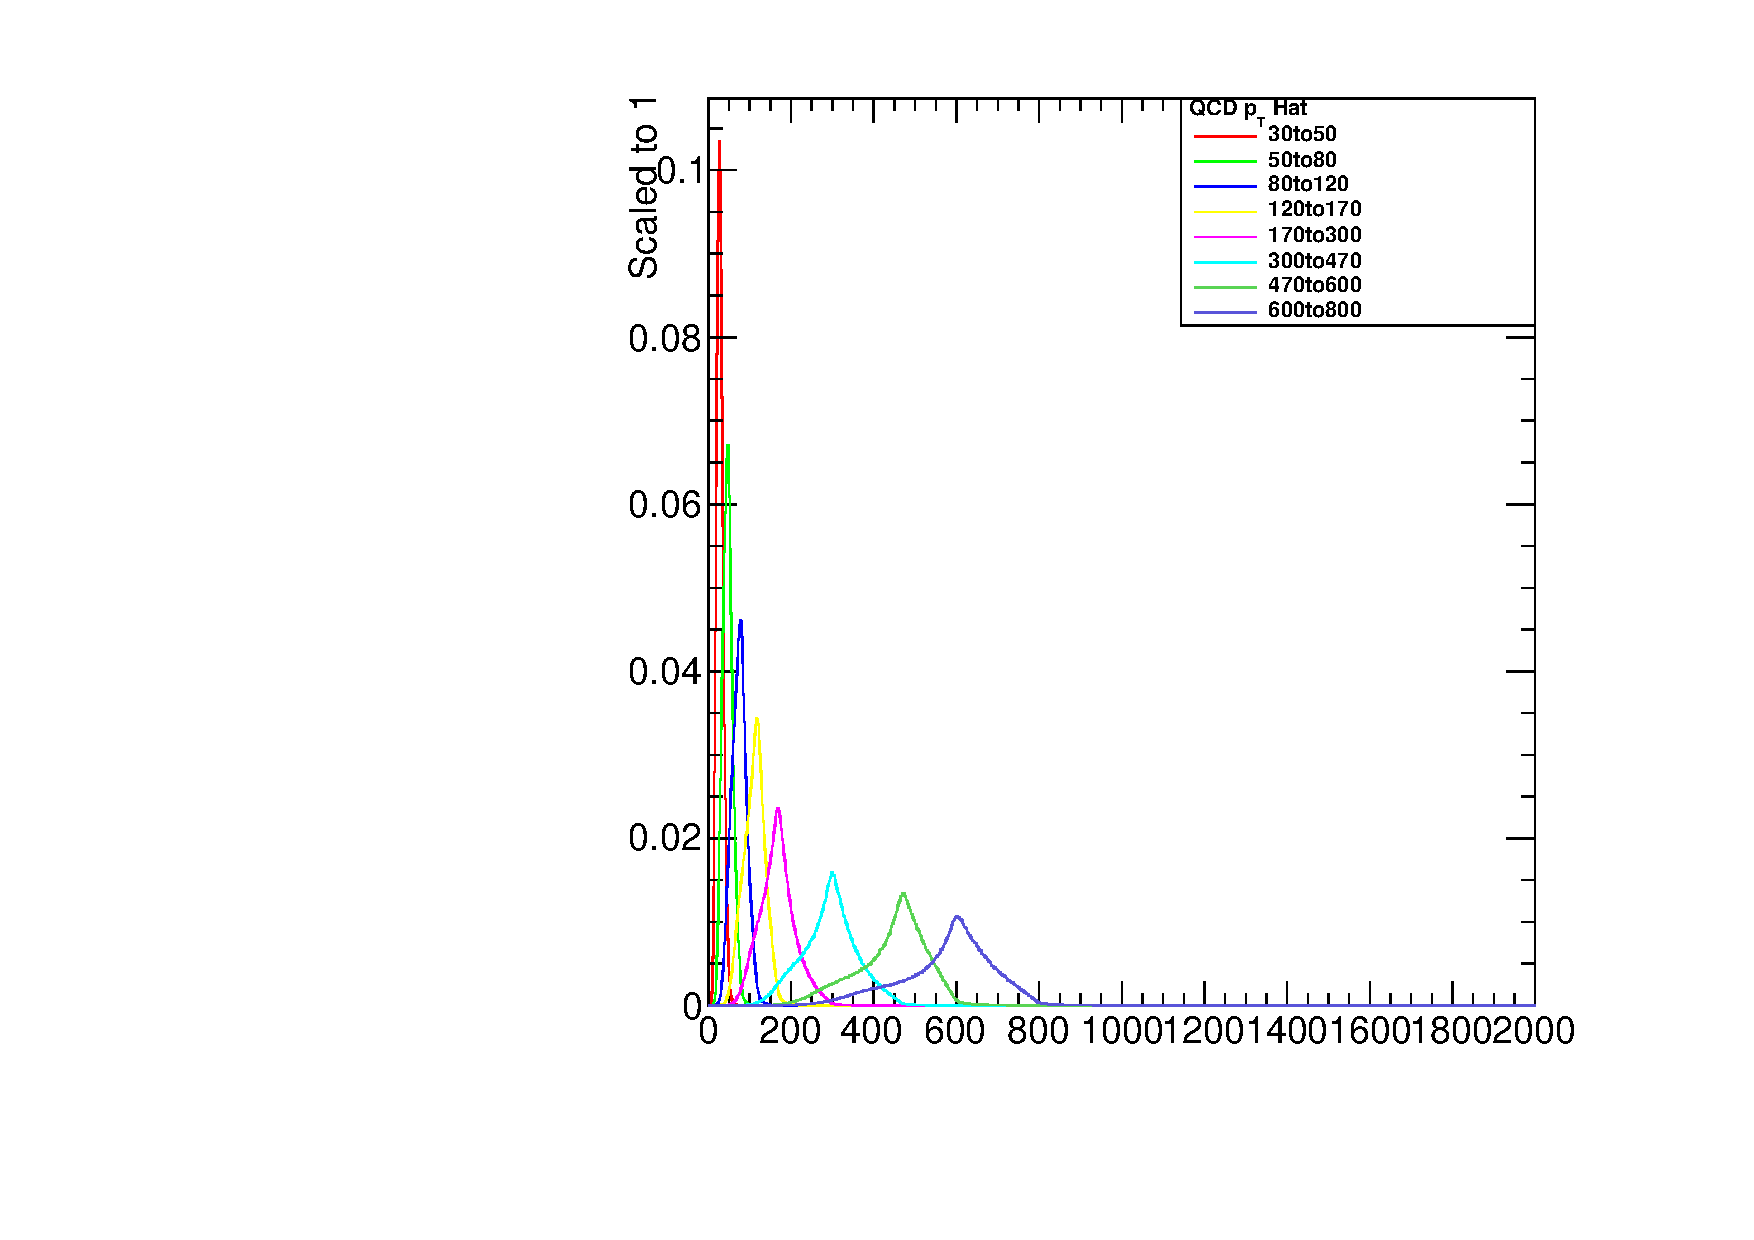
\includegraphics[width=1.0\linewidth]{img/Jet1_Pt.pdf}
\end{minipage}

\begin{minipage}{.5\textwidth}
  \centering
  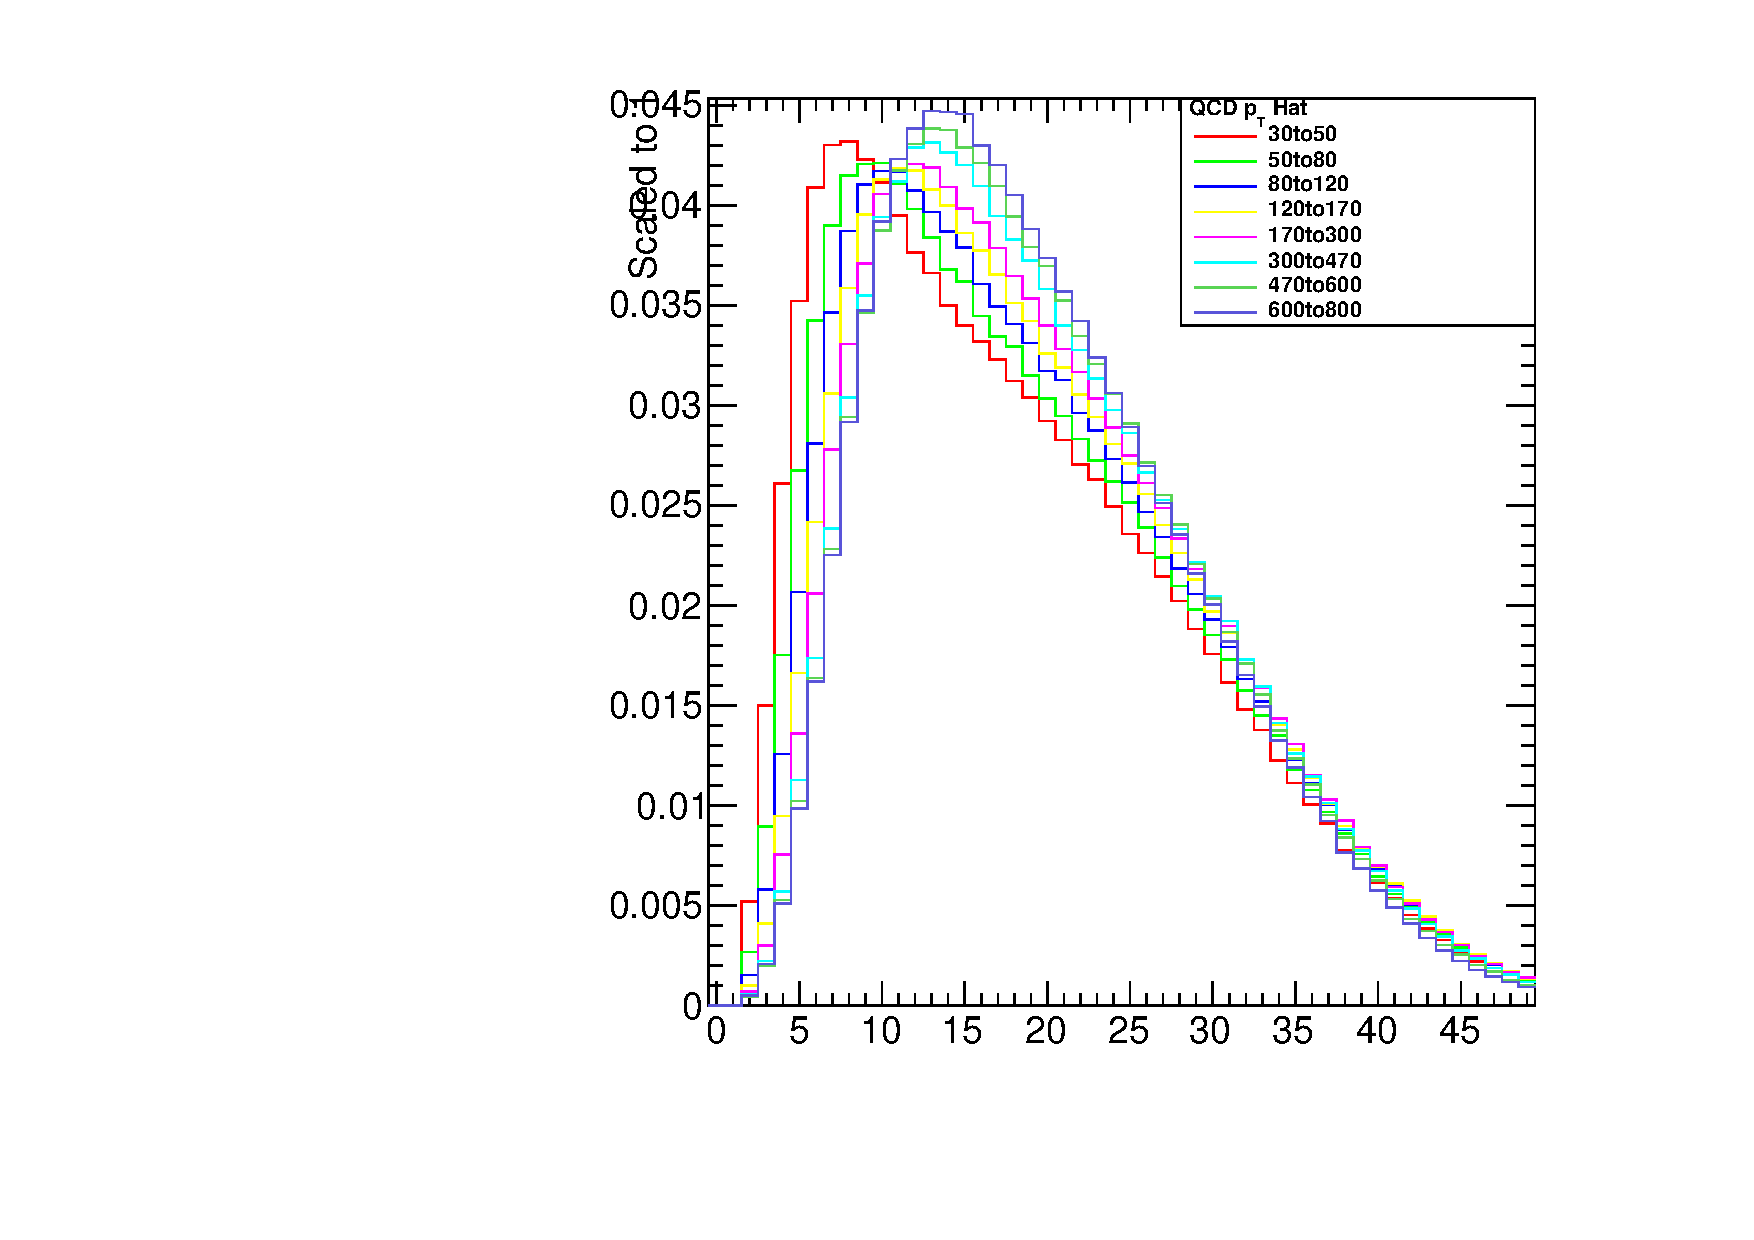
\includegraphics[width=1.0\linewidth]{img/Jets_Multiplicity.pdf}
\end{minipage}%
\begin{minipage}{0.5\textwidth}
  \centering
  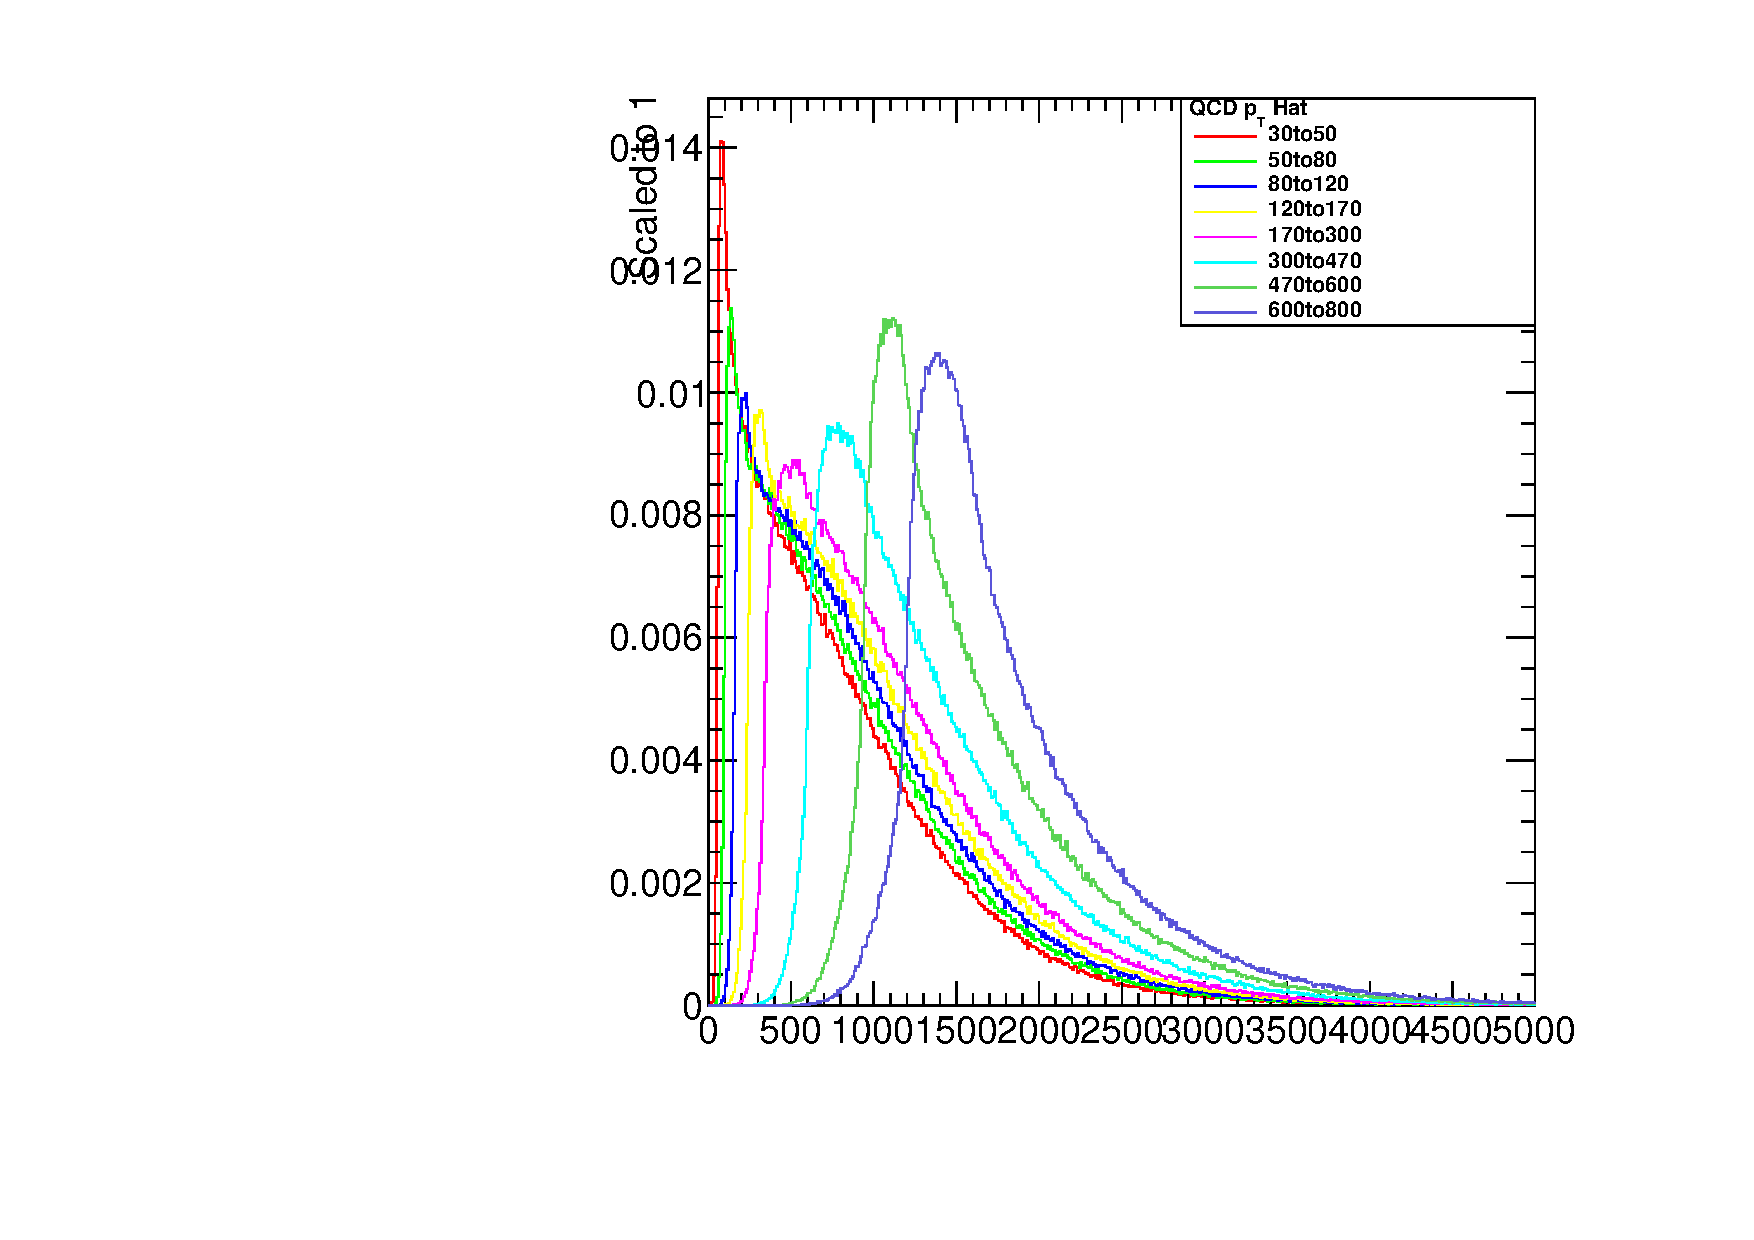
\includegraphics[width=1.0\linewidth]{img/Dijet_MaxMjj.pdf}
\end{minipage}

\begin{minipage}{.5\textwidth}
  \centering
  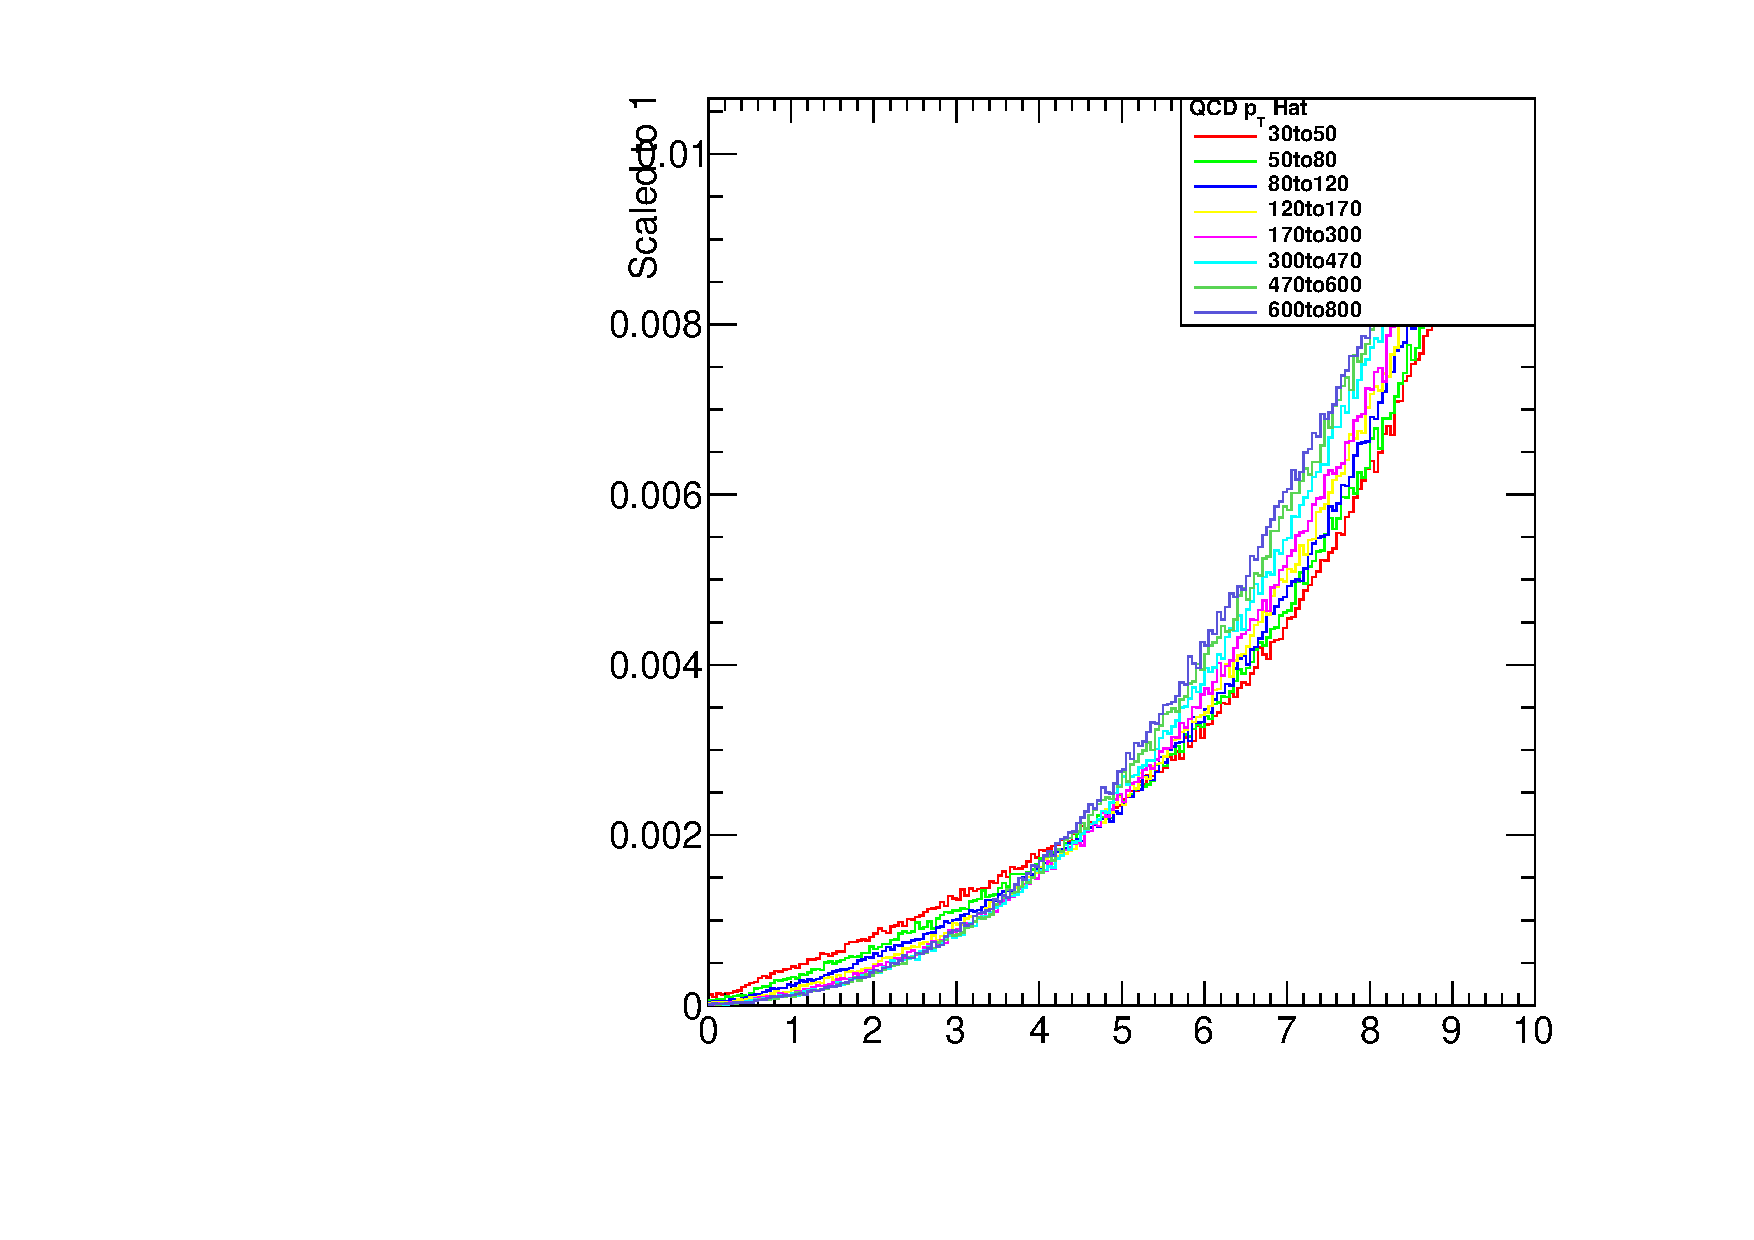
\includegraphics[width=1.0\linewidth]{img/Dijet_MaxDEta.pdf}
\end{minipage}%
\begin{minipage}{0.5\textwidth}
  \centering
  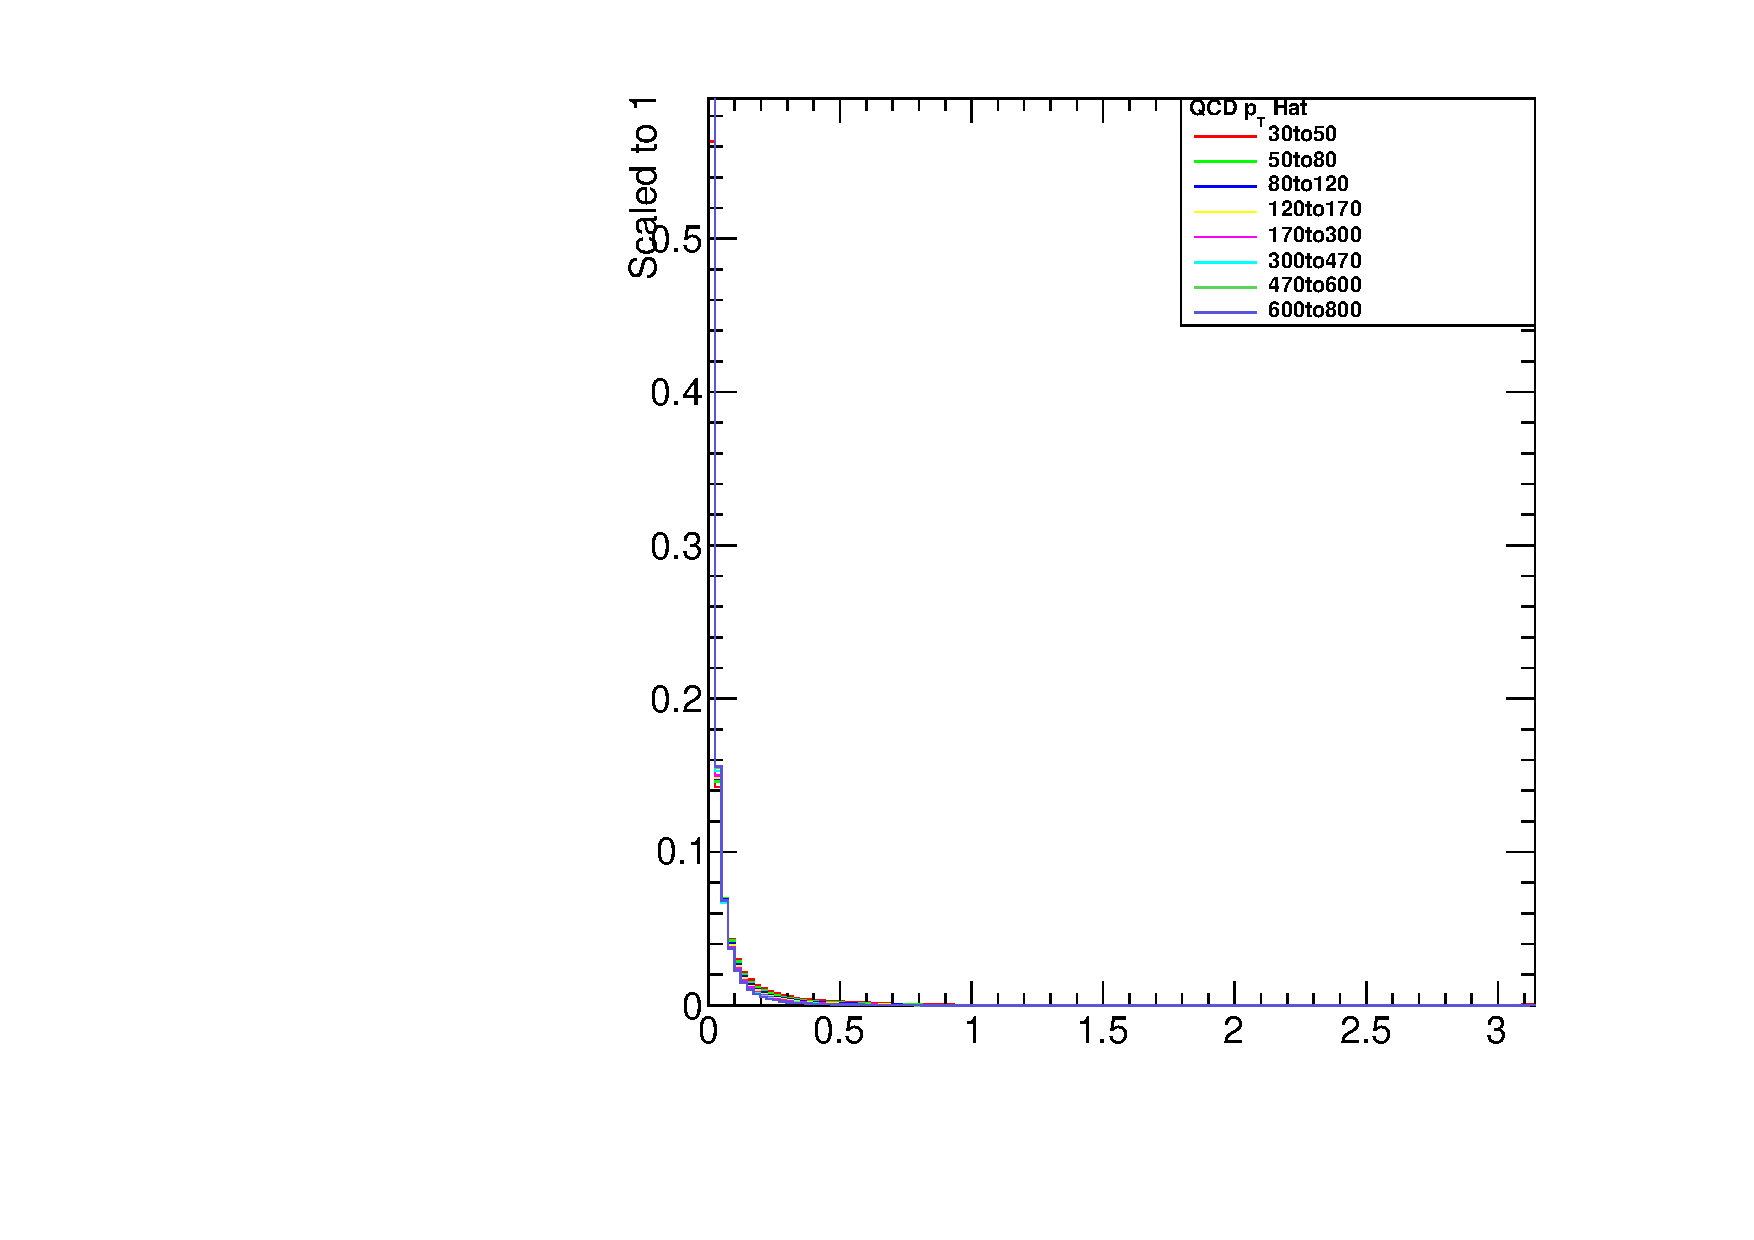
\includegraphics[width=1.0\linewidth]{img/Dijet_MinDPhi.pdf}
\end{minipage}


\section{Producing unfiltered events}

In order the understand the time cost of simulating events from scratch with CMSSW\_7\_2\_0\_patch1 configuration files were prepared using for each $p_\perp$ hat TODO
l
\begin{table}[htp]
\centering

\begin{tabular}{|c|c|l|c|c|}
\hline
\multicolumn{2}{|c|}{$p_\perp$ hat} & \multicolumn{3}{c|}{System Characteristics} \\
\hline
Min & Max & CPU Model & Core & RAM (kB) \\
\hline
\hline
 30 &  50 & Intel Core i7 9xx                         & 16 & 24023052 \\
 50 &  80 & Intel(R) Xeon(R) CPU E5-2650 v2 @ 2.60GHz & 32 & 62533844 \\
 80 & 120 & AMD Opteron(TM) Processor 6276            & 32 & 62533828 \\
120 & 170 & Intel(R) Xeon(R) CPU E5-2650 v2 @ 2.60GHz &  8 & 62533828 \\
170 & 300 & AMD Opteron(TM) Processor 6276            & 32 & 62533828 \\
300 & 470 & Intel(R) Xeon(R) CPU E5-2650 v2 @ 2.60GHz & 16 & 31225964 \\
470 & 600 & Intel(R) Xeon(R) CPU E5-2650 v2 @ 2.60GHz & 32 & 62533844 \\
600 & 800 & Intel Core i7 9xx                         & 16 & 24023052 \\
\hline	
\end{tabular}

\label{table_QCD_ProdUnfiltered_Hardware}
\end{table}


It should be noted th

\begin{table}[htp]
\centering

\begin{tabular}{|c|c||c|c||c|c|c|c||c|c|}
\hline
\multicolumn{2}{|c|}{$p_\perp$ hat} & \multicolumn{2}{|c||}{Job Times} & \multicolumn{4}{c||}{CPU Times} & \multicolumn{2}{c|}{Size (MB)} \\
\hline
Min & Max & Total & Avg Event & Total & Total Event & Avg Event & Non-Event   & Job & Avg Event \\
\hline
\hline
 30 &  50 & 9985.93 & 99.8593 & 7520.65 & 7394.73 & 73.9473 & 125.92 & 128 & 1.28 \\
 50 &  80 & 10769.5 & 107.695 & 7462.92 & 7369.9  & 107.695 &  93.02 & 132 & 1.32 \\
 80 & 120 & 16576.5 & 165.765 & 12902   & 12739.3 & 127.393 &  162.7 & 144 & 1.44 \\
120 & 170 & 10942.9 & 109.429 & 8302.49 & 8216.92 & 82.1692 &  85.57 & 152 & 1.52 \\
170 & 300 & 18225.8 & 182.258 & 14636.6 & 14475.7 & 144.757 &  160.9 & 165 & 1.65 \\
300 & 470 & 13346.1 & 133.461 & 11611.5 & 11523.6 & 115.236 &   87.9 & 177 & 1.77 \\
470 & 600 & 15774.7 & 157.747 & 13511.4 & 13413.7 & 134.137 &   97.7 & 189 & 1.89 \\
600 & 800 & 16422.1 & 164.221 & 15851.5 & 15726.5 & 157.265 &    125 & 192 & 1.92 \\
\hline
\hline
\multicolumn{2}{|l|}{Average} & 14005 & 140.05 & 11474.9 & 11357.5 & 117.8 & 117.3 &  &  \\
\hline
\end{tabular}

\caption{Step 1}
\label{table_QCD_ProdUnfiltered_Step1}
\end{table}

% -rw-r--r--. 1 pela zh 128M Apr 12 03:12 QCD_Pt-30to50_step1.root
% -rw-r--r--. 1 pela zh 132M Apr 12 03:24 QCD_Pt-50to80_step1.root
% -rw-r--r--. 1 pela zh 144M Apr 12 05:01 QCD_Pt-80to120_step1.root
% -rw-r--r--. 1 pela zh 152M Apr 12 03:28 QCD_Pt-120to170_step1.root
% -rw-r--r--. 1 pela zh 165M Apr 12 05:28 QCD_Pt-170to300_step1.root
% -rw-r--r--. 1 pela zh 177M Apr 12 04:06 QCD_Pt-300to470_step1.root
% -rw-r--r--. 1 pela zh 189M Apr 12 04:48 QCD_Pt-470to600_step1.root
% -rw-r--r--. 1 pela zh 192M Apr 12 04:59 QCD_Pt-600to800_step1.root


% -rw-r--r--. 1 pela zh  30M Apr 12 03:34 QCD_Pt-30to50_step2.root
% -rw-r--r--. 1 pela zh  32M Apr 12 03:51 QCD_Pt-50to80_step2.root
% -rw-r--r--. 1 pela zh  34M Apr 12 05:50 QCD_Pt-80to120_step2.root
% -rw-r--r--. 1 pela zh  35M Apr 12 03:56 QCD_Pt-120to170_step2.root
% -rw-r--r--. 1 pela zh  37M Apr 12 06:22 QCD_Pt-170to300_step2.root
% -rw-r--r--. 1 pela zh  39M Apr 12 05:04 QCD_Pt-300to470_step2.root
% -rw-r--r--. 1 pela zh  40M Apr 12 05:37 QCD_Pt-470to600_step2.root
% -rw-r--r--. 1 pela zh  41M Apr 12 05:49 QCD_Pt-600to800_step2.root


\begin{table}[htp]
\centering

\resizebox{\linewidth}{!}{
\begin{tabular}{|c||c|c|c|c||c|c|}
\hline
 & \multicolumn{4}{c||}{CPU Times} &  \\
\hline
$p_\perp$ hat & Total & Total Event & Avg Event & Non-Event   & Ev. Size (MB) \\
\hline
\hline
  30-50 & 1074.55 & 1023.63 & 10.2363 & 50.92 & 0.30 \\
  50-80 & 1163.04 & 1108.85 & 11.0885 & 54.19 & 0.32 \\
 80-120 & 2395.97 & 2308.39 & 23.0839 & 87.58 & 0.34 \\
120-170 & 1276.21 & 1232.36 & 12.3236 & 43.85 & 0.35 \\
170-300 & 2632.94 & 2548.5  & 25.485  & 84.44 & 0.37 \\
300-470 & 1832.55 & 1776.45 & 17.7645 & 56.1  & 0.39 \\
470-600 & 2130.65 & 2055.35 & 20.5535 & 75.3  & 0.40 \\
600-800 & 2726.66 & 2658.05 & 26.5805 & 68.61 & 0.41 \\
\hline
\hline
Average & 2269.0 & 1838.9 & 18.4 & 65.1 & 0.36 \\
\hline
\end{tabular}
}

\label{table_QCD_ProdUnfiltered_Step2}
\end{table}


\section{Generator level filters}

Two generator level filters were developed to preform this studies/productions. They filtered event on the generator jets and MET.

\subsection{Generator Jets Filter}

TODO: Description of the generator jet filter

\subsection{Generator MET Filter}

TODO: Description of the generator MET filter 

\newpage
\appendix
\section{Code Setup}

To reproduce this study you need to create a new CMSSW area, clone the git repository and get some configuration files from a remote server. To do this issue the following commands in a lxplus (SLC6) bash terminal:

\lstset{
  language=bash,
  basicstyle=\footnotesize, 
  breaklines=true
}
\begin{framed}
\begin{lstlisting}
cmsrel CMSSW_7_2_0_patch1
cd CMSSW_7_2_0_patch1/src/
cmsenv
git clone git@github.com:joaopela/VBFHiggsToInvisible.git
git checkout !!!TODO!!! <tag>
./VBFHiggsToInvisible/SampleProduction/scripts/getConfigFiles.sh
scramv1 b -j 5
\end{lstlisting}
\end{framed}

The configuration files are located at:

\begin{framed}
\begin{lstlisting}
VBFHiggsToInvisible/SampleProduction/test/13TeV/VBFQCD/
\end{lstlisting}
\end{framed}

\newpage
\section{Code Simulation}

Below the cmsDriver.py code to generate the CMSSW configuration files to generate unfiltered QCD samples in the $p_\perp$ hat of 30 to 50 GeV. This generation/simulation has been made over two steps. 

Step one comprises:
\begin{itemize}
  \item GEN: Actual physics process simulation
  \item SIM: Geant simulation of the intereaction of particles with the detector
  \item DIGI: Simulation of the response of CMS electronics
  \item L1: Simulation of the Level 1 Trigger
  \item DIGI2RAW: Conversion of the Digital Signal back to ``raw'' signal
  \item HLT:GRun: High Level Trigger Simulation
\end{itemize}


\lstset{
  language=bash,
  basicstyle=\footnotesize, 
  breaklines=true
}
\begin{framed}
\begin{lstlisting}
cmsDriver.py Configuration/GenProduction/python/BTV-Fall13-00042-fragment.py 
  --mc 
  --fileout file:QCD_Pt-30to50_step1.root 
  --eventcontent RAWSIM 
  --customise SLHCUpgradeSimulations/Configuration/postLS1Customs.customisePostLS1,Configuration/StandardSequences/SimWithCastor_cff.customise 
  --datatier GEN-SIM-RAW 
  --pileup_input "dbs:/MinBias_TuneA2MB_13TeV-pythia8/Fall13-POSTLS162_V1-v1/GEN-SIM" 
  --pileup 'AVE_35_BX_50ns,{"N":30}' 
  --conditions PHYS14_ST_V1 
  --step GEN,SIM,DIGI,L1,DIGI2RAW,HLT:GRun 
  --magField 38T_PostLS1 
  --geometry Extended2015 
  --python_filename QCD_Pt-30to50_step1_cfg.py 
  --no_exec 
  -n 100
\end{lstlisting}
\end{framed}

Step one comprises:
\begin{itemize}
  \item RAW2DIGI: Simulation of RAW to DIGI process
  \item L1Reco: Reconstruction of Level 1 trigger quantities
  \item RECO: Reconstruction of the event
\end{itemize}

\begin{framed}
\begin{lstlisting}
cmsDriver.py step2 
  --mc 
  --filein file:QCD_Pt-30to50_step1.root 
  --fileout file:QCD_Pt-30to50_step2.root 
  --eventcontent AODSIM 
  --customise SLHCUpgradeSimulations/Configuration/postLS1Customs.customisePostLS1,Configuration/DataProcessing/Utils.addMonitoring 
  --datatier AODSIM 
  --conditions PHYS14_ST_V1 
  --step RAW2DIGI,L1Reco,RECO 
  --magField 38T_PostLS1 
  --python_filename QCD_Pt-30to50_step2_cfg.py 
  --no_exec 
  -n 100
\end{lstlisting}
\end{framed}

\newpage
\begin{thebibliography}{10}

\bibitem{FirstReference}

\end{thebibliography}

\end{document}
